%!TEX root = ../Thesis.tex
\chapter{Introduction}\label{cha:introduction}
%


\todo[inline]{
This introductory chapter will briefly provide context for the material/results presented in this report and give motivation and a description of the problem to be solved. A literature review summarises existing relevant knowledge and establishes the foundation of the later control system. The scope of the work is then defined through a list of assumptions. Finally, the contributions of the thesis are defined and elaborated.}



\section{Motivation}\label{sec:motivation}

Combustion of Municipal Solid Waste(MSW) is a process that has gained increased attention in the last years. This is both as a result of a steady increase in produced waste, as well as stricter regulations, which means that the plants have to follow stricter standards with regards to both gas emission and management of the solid ash left behind after the combustion. One way to ensure all conditions are met is to find some operating point that is know for causing the system to behave in the desired manner, and then using a controller to make sure the system stays near that state, regardless of any disturbances that may affect the process. A solution using cascaded PID-controllers has already been made by SINTEF. But that model will not be able to take full advantage of how to combine different inputs in such a way disturbances are suppressed, while not affecting other outputs too much. 

\subsection{Literature review}
There has already been quite a bit on work on the subject of waste incineration, like in \cite{waste_prof}. Furthermore, there has been some interest in using additional sensors to the ones that are normally used when controlling such a plant. In \cite{summer_student}, an estimate of the heating value was used to give a controller that could handle changes in waste-quality more effectively. \cite{waste_prof} tested several different implementations for how to control waste-combustion plants. Waste-incineration suffers from the typical problem that when one tries to increase one of the measured variables by increasing one of the inputs, there will usually be a rather large overshoot, as well as some states decreasing before they start to increase again. This is what is known as a non-minimum phase system and they are usually more difficult to control. Furthermore, changing one input usually affects all outputs. This makes it so that there are other controllers than PID-controllers that may be able to give better results. This thesis will attempt to improve on the solution in \cite{summer_student} by estimating a system with the method given in \cite{ERA_source}, and then combining the acquired model with standard linear dynamical systems theory, like what is found in \cite{cont_LQR_lecture} to make a better controller. Finally, the estimated model may also be used for gaining a feeling for how sensitive the rest of the system is to disturbances, measurement  and modelling errors. The method will be repeated on a selection of different model-based linear controllers with slightly different architecture  to find the one that has the best performance while also having some indicator of its robustness. 
\todo[inline]{Make sure I do this...}

\subsection{Assumptions}
Since the main implementation is based on a linear model, the biggest assumption about the plant is that it behaves sufficiently similar to a linear time-invariant system. Furthermore, it is assumed that any time-delay in the control-loop remains within certain borders. Additionally, it is assumed that all modelling errors are on the form of pure time-delays or in the form of incorrect scaling for the input-matrix $B$, and that these errors vary so slowly that they can be seen as piece-wise constant when stabilising the plant and that these periods are so long that the controller gets the time to stabilise the plant. The implementation that was used also assumes that the process disturbances have a much larger effect on measured signals than the measurement-noise as long as a low-pass filter with a cutoff-frequency of $1 \left[\frac{rad}{s}\right]$ is used. However, this assumption can be changed later by using a new filter and re-tuning the weights in the controller and the state estimator. 
\subsection{Contributions}
The contributions from this project mainly come in the form of implementations of the different controllers, as well as an implementation of the Eigensystem Realisation Algorithm. All steps needed for the algorithm to work can be found in \cite{ERA_source}. Two different estimated systems were implemented. One that only considers how the controlled disturbances affect the outputs, and one that also uses the measured disturbances from the simulation to give an optimistic estimate of the increase in performance if they could be measured. It can also be used for getting a better estimate of how the process-disturbances affect the output, which can be used when designing the estimator. 

\noindent
Making a Linear Quadratic Estimator that is decoupled form the rest of the controller also allows for properly utilising the sensor measurements for state-estimation, since a Model Predictive Controller needs more computation time than a Kalman filter. 
\noindent
Finally, some different controller architectures were explored, which had the purpose of making the controller follow the desired steady-state, since some combinations of inputs can only be allowed to handle transient inputs, and should not be used to make the controller reach its steady-state. Finally, some robustness analysis was also done on the linear, estimated system to give some kind of guess to how robust the controller might be. 

\subsection{Outline}
The thesis is divided into $N$ chapters. 

\begin{itemize}
  \item \ref{cha:process_overview}: Process overview 
  \item \ref{cha:characteristics_of_process}: Features of the process 
  \item \ref{sec:ERA}: Parameter estimation
  \item \ref{cha:controllers}: Controllers
  \item \ref{cha:experimental_results}: Experimental result
  \item \ref{cha:conclusions}: Conclusion and future work
\end{itemize}




Chapter \ref{cha:process_overview} will explain what happens in the process, without going in-depth about what mathematical model is required to simulate the given system. This is mostly due to the complexity of a combustion process, which results in a proper explanation of how the process works being outside the scope of this thesis. 


\noindent
Chapter \ref{cha:characteristics_of_process} will cover the qualitative properties of the system's step responses when the system is excited around the operating point. This may give some information as to what issues will be the most pressing when trying to control the plant. 


\noindent
The different controller architectures will be discussed in chapter \ref{cha:controllers}, namely two PID-controller architectures, as well a few methods for optimal control. Namely, the Model Predictive Controller and the Linear Quadratic Regulator. Different architectures can be tested, depending on if there is supposed to be some kind of cost on the system for excessively increasing the primary air while reducing the secondary air. 


\noindent
Chapter \ref{cha:experimental_results} describes the process of tuning the controllers, as well as how the resulting closed-loop system respond to disturbances and noise. Because of the system being somewhat inaccurate when it comes to representing how the system will most likely act in reality. 
\todo[inline]{Add a part where all disturbances can be measured (?)}
\noindent
Finally, Chapter \ref{cha:conclusions} covers suggestion for future work that could expand and improve the results of the current project. 

% What is the motivation for considering the problems/question that you approach in your work? Why is this an interesting problem? The motivation should instead describe why it is interesting from a societal point of view, and/or from a scientific point of view.}
% \todo[inline]{Remember to cite what has been done earlier on the topic, to put your work in the correct context: In \cite{Adaptiv_boken} a control law is defined which..., while \cite{Adaptiv_boken} considers the particular case of... However, in these works... and in this work, we will extend this by... / we will instead... In "Reference to your own pre-project" a literature review was performed, showing that there is a need for ... }
% \todo[inline]{Moreover, a preliminary controller was developed... but has the drawback that... In this thesis, we will instead ... / we will further develop this control law by utilising the control method XX... 
% }
% Figures are referred to as follows: In Fig.~\ref{fig:curve} you see an interesting curve. There is also a table in this sample report: Table~\ref{tab:a-table}.

% \subsection{A Subsection}\label{ssec:a-subsection}


% \subsubsection{A Subsubsection}\label{sssec:a-subsubsection}

% \lipsum[2]

% \begin{figure}[htbp]
%   \centering
%   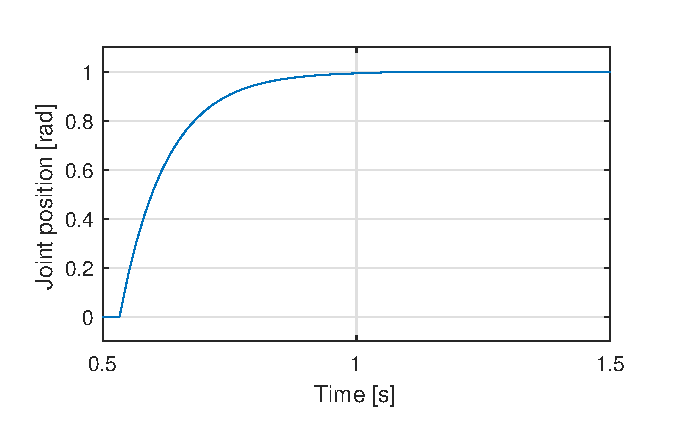
\includegraphics[width=.7\textwidth]{img/time-constant}
%   \caption{The time evolution of the joint angle $q$}
%   \label{fig:curve}
% \end{figure}

% \begin{table}[htbp]
%   \centering
%   \caption{A table}
%   \begin{tabular}{cc}
%     \toprule
%     Something & Something else \\
%     \midrule
%     A & a \\
%     B & b \\
%     \bottomrule
%   \end{tabular}
%   \label{tab:a-table}
% \end{table}

% \section{Literature review}\label{sec:review}

% \section{Assumptions}\label{sec:assumptions}
% Include this section if it is necessary to state some assumptions that you have made to restrict the scope of the thesis.

% \section{Contributions}\label{sec:contributions}
% Here you describe the main contributions of your work: What are the new results - the achievements - of your work on the master project. For instance:
% The main contributions of the work presented in this thesis are as follows:
% \begin{itemize}
% 	\item The development of a control law for ...
% 	\item The development of a simulator for...
% 	\item A simulation study evaluating the performance of the proposed control method.
% 	\item Experimental validation of the theoretical results, using the autonomous ground vehicle...
% \end{itemize} 
% Elaborate on each item/contribution - this is an opportunity for you to convey to the reader (and the examiner) all that you have done during your master´s project work.

% \section{Outline}\label{sec:outline}
% The report is organized as follows. In Chapter~\ref{cha:characteristics_of_process} a mathematical model is developed to describe the system... In Chapter

          
